\documentclass[fleqn,11pt]{ExcelAtFIT} % Document font size and equations flushed left

\usepackage[font={normalsize}]{subfig}
\usepackage{array}
\usepackage{multirow}
\usepackage{multicol}
\usepackage{dblfloatfix}

\colorlet{fixme}{green!50!black}
\newcommand{\fixme}[1]{{\color{fixme} {{\textbf{[FIXME]}} #1} }}

\colorlet{sos}{red}
\newcommand{\sos}[1][]{{\color{sos} {{[ \textbf{???}} #1]} }}

\colorlet{grayintable}{black!50}

\newcommand{\uv}[1]{\quotedblbase #1\textquotedblleft}

%--------------------------------------------------------
%--------------------------------------------------------
%	REVIEW vs. FINAL VERSION
%--------------------------------------------------------

%   LEAVE this line commented out for the REVIEW VERSIONS
%   UNCOMMENT this line to get the FINAL VERSION
%\ExcelFinalCopy


%--------------------------------------------------------
%--------------------------------------------------------
%	LANGUAGE
%--------------------------------------------------------
%   Recommended language for Excel@FIT paper is English.
%   However, in emergency, you can write in Czech or Slovak.
%   In such a case, uncomment one of these lines to localize the template.
%--------------------------------------------------------
%\ExcelSlovakLabels
\ExcelCzechLabels


%--------------------------------------------------------
%--------------------------------------------------------
%	PDF CUSTOMIZATION
%--------------------------------------------------------

\hypersetup{
	pdftitle={Souběžné učení v koevolučních algoritmech},
	pdfauthor={Michal Wiglasz},
	pdfkeywords={Keyword1, Keyword2, Keyword3}
}


%--------------------------------------------------------
%--------------------------------------------------------
%	ARTICLE INFORMATION
%--------------------------------------------------------

\ExcelYear{2015}

\PaperTitle{Souběžné učení v koevolučních algoritmech}

\Authors{Michal Wiglasz*}
\affiliation{*%
  \href{mailto:xwigla00@stud.fit.vutbr.cz}{xwigla00@stud.fit.vutbr.cz},
  \textit{Fakulta informačních technologií, Vysoké učení technické v Brně}}
%%%%--------------------------------------------------------
%%%% in case there are multiple authors, use the following fragment instead
%%%%--------------------------------------------------------
%\Authors{Jindřich Novák*, Janča Dvořáková**}
%\affiliation{*%
%  \href{mailto:xnovak00@stud.fit.vutbr.cz}{xnovak00@stud.fit.vutbr.cz},
%  \textit{Faculty of Information Technology, Brno University of Technology}}
%\affiliation{**%
%  \href{mailto:xdvora00@stud.fit.vutbr.cz}{xdvora00@stud.fit.vutbr.cz},
%  \textit{Faculty of Information Technology, Brno University of Technology}}

\Keywords{
Koevoluční algoritmus ---
Kartézské genetické programování ---
Evoluční algoritmus ---
%Baldwinův efekt ---
Plasticita fitness ---
Predikce fitness ---
Zpracování obrazu
}

\Supplementary{\sos}
%\Supplementary{\href{http://youtu.be/S3msCdn3fNM}{Ukázkové video} --- \href{http://excel.fit.vutbr.cz/}{Zdrojové kódy}}


%--------------------------------------------------------
%--------------------------------------------------------
%	ABSTRACT and TEASER
%--------------------------------------------------------

\Abstract{
U kartézského genetického programování (CGP) je časově nejnáročnější vyhodnocení kvality kandidátních řešení. Bylo ukázáno, že je možné evoluci urychlit pomocí koevoluce s prediktory fitness, které slouží k přibližnému určení kvality kandidátních řešení. Nevýhodou koevoluce je nutnost provést mnoho časově náročných experimentů pro určení nejvýhodnější velikosti prediktoru pro daný problém. V tomto článku je představena nová reprezentace prediktorů fitness s plastickým fenotypem, založená na principech souběžného učení v evolučních algoritmech. Plasticita fenotypu umožňuje odvodit různé fenotypy ze stejného genotypu. Díky tomu je možné adaptovat velikost prediktoru na současný průběh evoluce a obtížnost řešeného problému. Z experimentů vyplývá, že lze dosáhnout srovnatelné kvality jako u standardního CGP při kratší době běhu programu a zároveň odpadá nutnost hledání nejvýhodnější velikosti prediktoru.
}

\Teaser{
	\TeaserImage{teaser.pdf}
	\TeaserImage{teaser.pdf}
	\TeaserImage{teaser.pdf}
}



%--------------------------------------------------------
%--------------------------------------------------------
%--------------------------------------------------------
%--------------------------------------------------------
\begin{document}

\startdocument


%--------------------------------------------------------
%--------------------------------------------------------
%	ARTICLE CONTENTS
%--------------------------------------------------------

%--------------------------------------------------------
%--------------------------------------------------------
%--------------------------------------------------------
%--------------------------------------------------------
\section{Úvod}

Genetické programování umožňuje automatizovaně vytvářet programy s~požadovaným chováním, které je definováno v \emph{trénovací množině}. Každý prvek této množiny reprezentuje jeden \emph{případ fitness} a skládá se ze vstupních hodnot programu a požadovaných výstupních hodnot. U~složitějších problémů může být takových případů fitness velmi mnoho. Protože výpočet fitness je časově nejnáročnější částí evoluce, je vhodné do trénovací množiny zahrnout pouze část případů fitness a urychlit tak výpočet. Na druhou stranu je třeba velikost množiny a používané případy fitness zvolit tak, aby byl program dostatečně obecný a i pro kombinace vstupů neobsažené v~trénovací množině byly výstupy programu dle požadavků.

Vhodné případy fitness lze zvolit například pomocí genetického algoritmu. Evoluce podmnožin případů fitness může probíhat souběžně s hledáním řešení problému. Byla představena koevoluce s prediktory fitness v genetickém progamování se stromovou reprezentací programů \cite{Schmidt} i kartézském genetickém programování \cite{SikuEuroGP}. Nevýhodou je fixní velikost prediktorů, kterou je třeba stanovit předem, což mnohdy nejde jinak než experimentálně. Tento nedostatek lze řešit nepřímým kódováním prediktorů, kdy se vyvíjí funkce generující posloupnost ukazatelů do trénovací množiny \cite{SikuHulva}.

Cílem práce je navrhnout a experimentálně vyhodnotit koevoluci CGP a přímo kódovaných prediktorů fitness s proměnlivou velikostí. Jejich velikost se adaptuje na řešený problém a stav evoluce kandidátních programů dle principů inspirovaných souběžným učením.

Tento článek má následující strukturu: v části \ref{sec:Coevolution} je představeno kartézské genetické programování a koevoluce s prediktory fitness. V části \ref{sec:AdaptiveSize} je představeno nové plastické kódování prediktoru a způsob adaptace jejich velikosti na řešený problém. V části \ref{sec:Experimental} je navržený algoritmus vyhodnocen a srovnán se standardním CGP a s koevolucí CGP a prediktorů fixní velikosti.



%--------------------------------------------------------
%--------------------------------------------------------
%--------------------------------------------------------
%--------------------------------------------------------
\section{Koevoluce prediktorů fitness v CGP}
\label{sec:Coevolution}

Kartézské genetické programování (CGP) představil Julian Miller koncem devadesátých let \cite{Miller2000}. V~CGP se programy kódují jako orientované acyklické grafy, reprezentované dvourozměrnou kartézskou mřížkou výpočetních uzlů (funkčních bloků) o rozměrech $n_c \times n_r$. Příklad kartézského programu je na obrázku \ref{fig:CgpCircuit}. Program má $n_i$ primárních vstupů a $n_o$ primárních výstupů. Každý ze vstupů funkčních bloků může být připojen k výstupu bloku o až $l$ sloupců nalevo nebo na některý z primárních vstupů programu. Každý z výpočetních uzlů provádí jednu $n_a$ možných funkcí, které jsou vybrány s ohledem na řešený problém. Každý primární výstup programu je připojen na výstup některého z funkčních bloků \cite{ZelenaCGP}.

\begin{figure}[h]
    \centering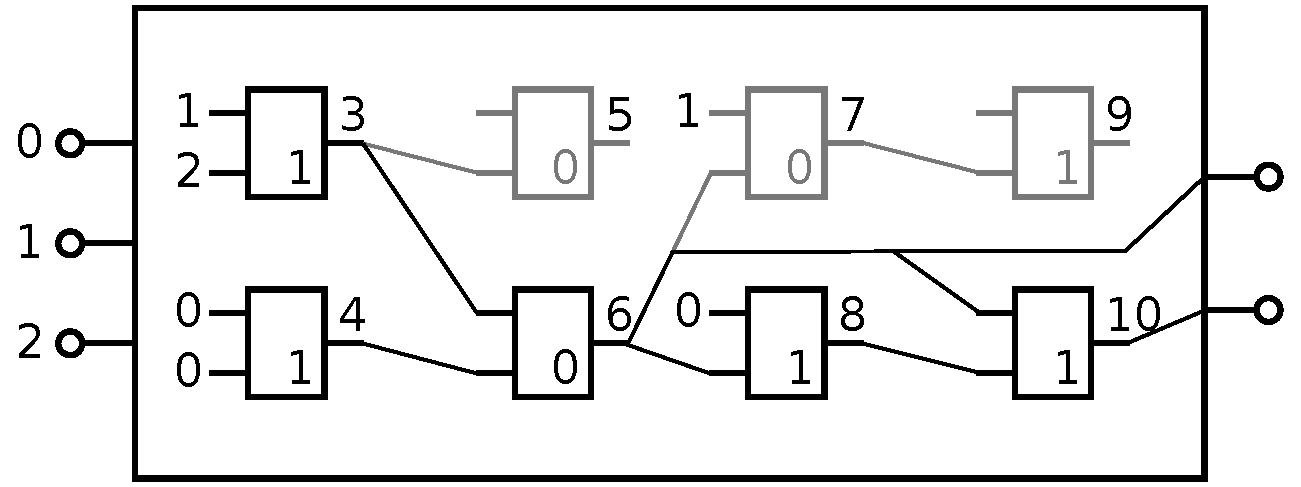
\includegraphics[width=\linewidth]{images/cgp.pdf}
    \caption{Program v~kartézském genetickém programování.}
    \label{fig:CgpCircuit}
\end{figure}

CGP bylo úspěšně použito v celé řadě úloh, jako je například návrh obrazových filtrů. Na vstup kartézského programu je přivedeno zvolené okolí pixelu, výstupem je filtrovaný pixel. Jako fitness funkce se používá například špičková hodnota poměru signál/šum v~decibelech (Peak Signal to Noise Ratio, PSNR):

\begin{equation}
    \label{eq:PSNR}
    \mathit{PSNR} = 10 \log_{10} \frac{255^2}{\frac{1}{MN} \sum\limits_{i,j} \left( v\left( i, j \right) - w\left( i, j \right)  \right)^2 }
\end{equation}

\noindent{}kde $M$ a $N$ označují rozměry obrázku, $v$ filtrovaný a $w$ původní obrázek \cite{ZelenaIF}.

Pro výpočet fitness kandidátního filtru musíme zpracovat celý obrázek, přičemž každý pixel můžeme považovat za jeden případ fitness. Protože i pro poměrně malé obrázky jich je několik tisíc, je výpočet fitness časově velmi náročný. Tento problém se dá řešit pomocí koevolučního algoritmu. Při koevoluci se souběžně vyvíjí několik různých populací, které mezi sebou interagují prostřednictvím fitness funkcí. Fitness jedince závisí kromě jeho fenotypu také i na jedincích z okolních populací. V případě koevoluce s prediktory fitness existují dvě populace a také archiv, do kterého jsou vkládána nejlepší nalezená kandidátní řešení. Řešení jsou vyvíjena pomocí CGP a jako fitness funkce slouží \textit{predikovaná fitness} $f_{\mathit{predicted}}$. Po vložení nového jedince do archivu se vypočítá i jeho skutečná fitness $f_{\mathit{exact}}$, pomocí které se ohodnocují prediktory fitness.

Druhá populace je tvořena prediktory fitness, což jsou podmnožiny množiny případů fitness. Jejich chromozomy jsou vektory ukazatelů do trénovací množiny o~konstantní délce. Potomci jsou tvořeni pomocí jednobodového křížení a mutace, kvůli zachování diverzity populace je několik potomků vytvořeno zcela náhodně. Využívá se i elitismus, kdy několik nejlepších jedinců rodičovské populace přechází do populace potomků. Fitness prediktoru je určena jako střední absolutní odchylka skutečné a predikované fitness všech programů v~archivu:

\begin{equation}
    \label{eq:fitnessPredictor}
    f \left( p \right) = \frac{1}{u} \sum\limits_{i=1}^{u} \left| f_{\mathit{exact}} \left( s \left( i \right) \right) - f_{\mathit{predicted}} \left( s \left( i \right) \right) \right|
\end{equation}

\noindent{}kde $p$ označuje prediktor, $s$ archiv programů obsahující $u$ jedinců. Prediktor s~nejnižší odchylkou je pak použit pro ohodnocování řešení z~populace kartézských programů.

Na začátku běhu programu jsou náhodně vytvořeny počáteční populace filtrů a prediktorů fitness. Poté je vypočtena skutečná fitness filtrů a nejlepší jedinec je umístěn do archivu. Pomocí něj jsou ohodnoceny prediktory fitness a je určen nejlepší z nich, který bude zpočátku sloužit pro výpočet predikované fitness. Po této inicializaci archivů pokračuje běh programu ve dvou oddělených vláknech, každé obsluhuje jednu populaci \cite{SikuPPSN}.

\begin{figure*}[t]
    \centering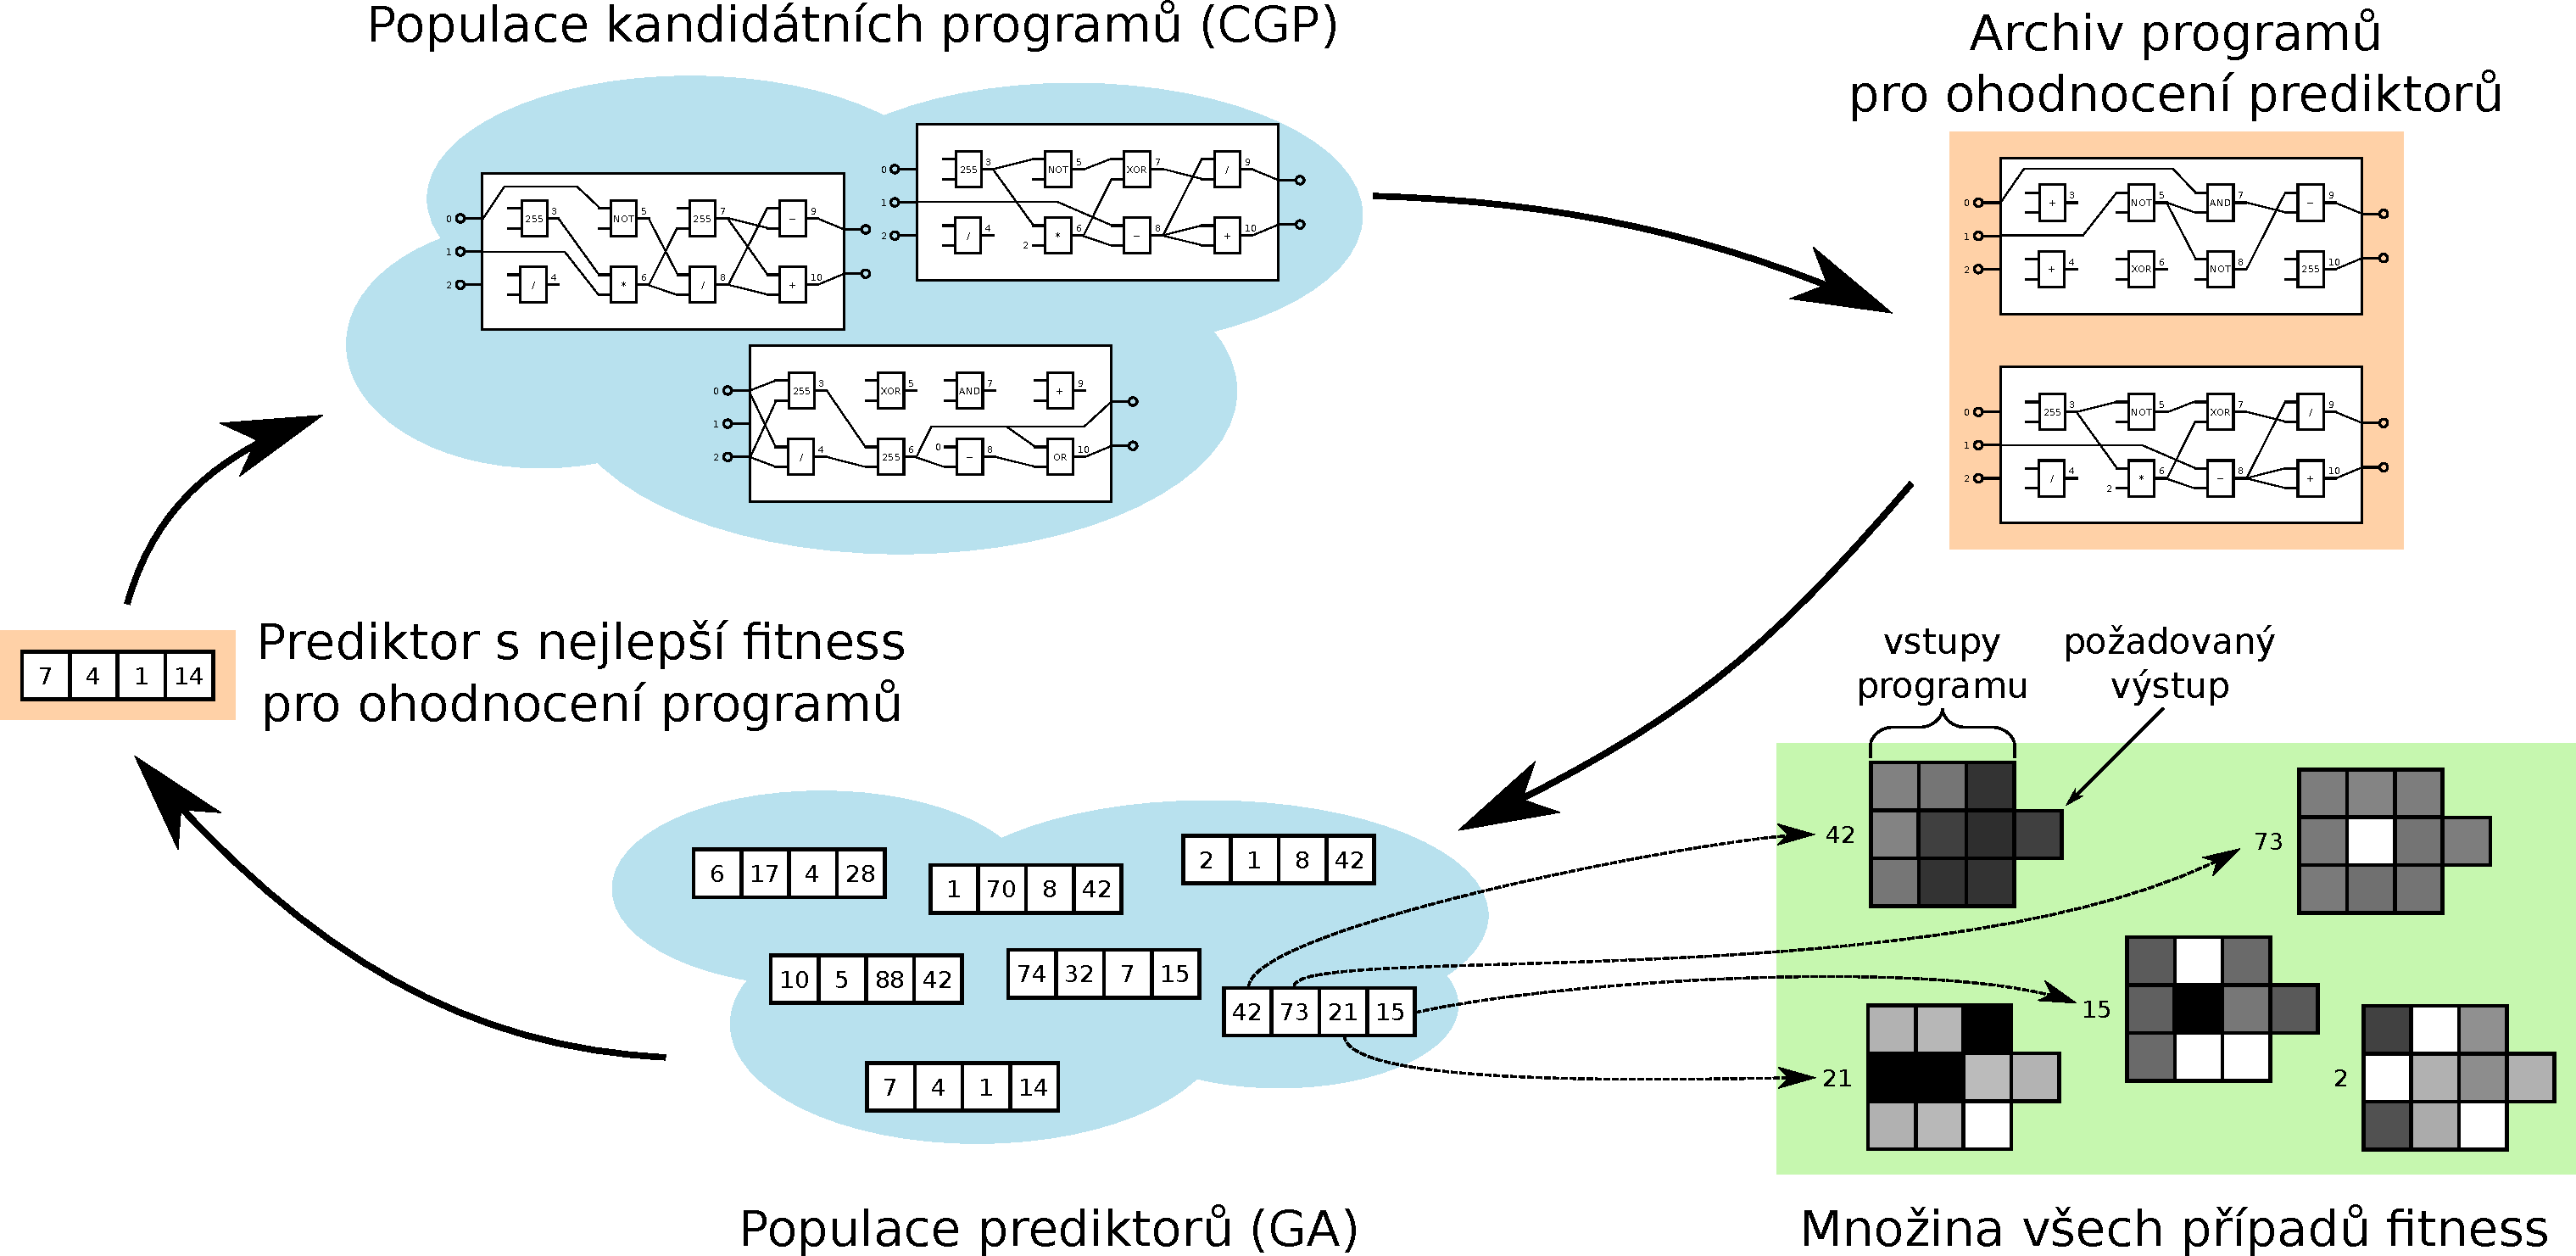
\includegraphics[width=0.9\linewidth]{images/coevolution-if.pdf}
    \caption{Schéma koevoluce CGP a prediktorů fitness.}
    \label{fig:CoevolutionScheme}
\end{figure*}



%--------------------------------------------------------
%--------------------------------------------------------
%--------------------------------------------------------
%--------------------------------------------------------
\section{Adaptivní velikost prediktorů fitness}
\label{sec:AdaptiveSize}

Nevýhodou koevolučního přístupu je nutnost stanovit velikost prediktoru. Ukazuje se, že pro různé problémy je výhodnější použít jinou velikost. Před použitím koevolučního CGP pro řešení nového problému je tedy nutné provést celou řadu experimentů, jejichž cílem je určit velikost prediktoru.

Cílem této práce je tento nedostatek překonat pomocí přímého kódování prediktorů s plastickým fenotypem, jehož velikost se může adaptovat na složitost řešeného problému. Plasticita je dosažena tím, že fenotyp netvoří všechny ukazatele obsažené v~genotypu, ale pouze jejich část. Fenotyp je z~genotypu tvořen postupným čtením genů od zvolené pozice (offsetu). Pokud hodnota (ukazatel do množiny případů fitness) právě čteného genu není obsažena ve fenotypu, je do něj vložena, v~opačném případě se gen ignoruje. Poté je přečten další gen a proces se opakuje. Během tvorby fenotypu nejsou čteny úplně všechny geny -- jejich počet je určen proměnnou \emph{UsedGenes}, která je součástí prostředí. Pokud je při čtení dosaženo konce genotypu, ale nebyl ještě přečten potřebný počet genů, pokračuje se od jeho začátku. Příklad tvorby fenotypu při použití šesti genů z~deseti ukazuje obrázek \ref{fig:PhenotypeContruction}.

\begin{figure}[h]
    \centering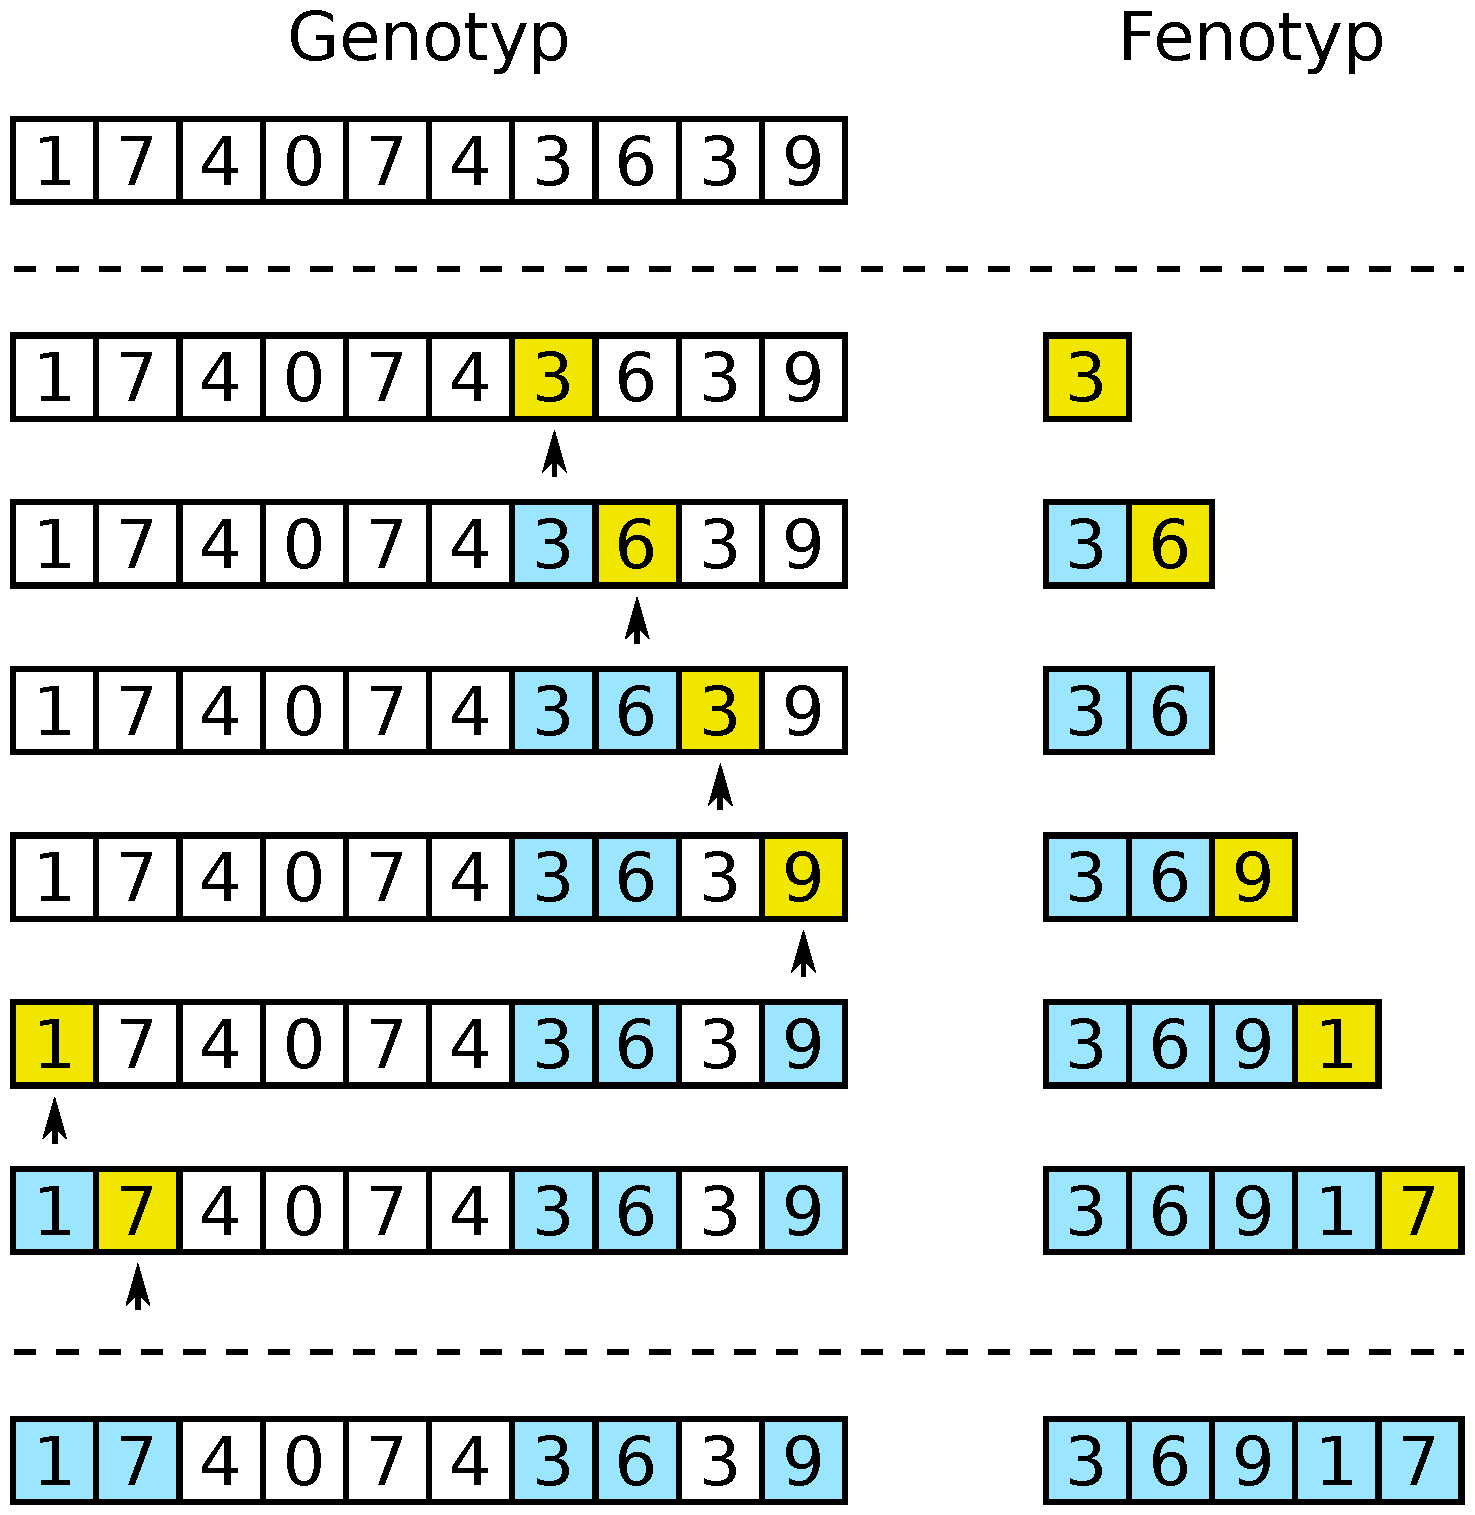
\includegraphics[width=0.85\linewidth]{images/phenotype.pdf}
    \caption{Postup konstrukce fenotypu prediktoru. Šipka označuje právě přečtený gen.}
    \label{fig:PhenotypeContruction}
\end{figure}

Adaptace velikosti prediktoru probíhá na základě sledování rychlosti vývoje skutečné fitness kandidátních řešení. Lze očekávat, že jejich populace prochází obdobími, kdy je celková schopnost adaptace vyšší (a fitness populace stoupá) a obdobími, kdy se adaptovat příliš nedokáže (a fitness se nemění). Důležitý je i směr změny fitness, protože je pro ohodnocení jedinců v CGP používána predikovaná fitness a skutečná fitness nejlepšího jedince může i klesat. Rychlost je určena jako podíl změny fitness nejlepšího jedince v populaci a počtu generací, které uběhly od poslední změny:

\begin{equation}
    \label{eq:velocity}
    v = \frac{\Delta{}f_{\mathit{exact}}}{\Delta{}G}
\end{equation}

Zároveň je sledována i přesnost prediktorů, protože u příliš krátkých prediktorů hrozí, že se velmi dobře adaptují na řešení uložené v archivu a nebudou dostatečně obecné. Nepřesnost prediktoru je vypočtena jako:

\begin{equation}
    \mathit{I} = \frac{f_{\mathit{predicted}}}{f_{\mathit{exact}}}
\end{equation}

Pro každou možnou situaci je určen koeficient, kterým je vynásobena současná hodnota proměnné \emph{UsedGenes}, čímž se změní velikost fenotypů prediktorů. Pravidla jsou tato:

\begin{itemize}
    \item Pokud je nepřesnost predikce příliš vysoká, prediktory se vždy prodlouží.
    \item Pokud fitness roste, prediktory se prodlouží a tím se zpřesní predikce. Rozlišuje se mezi \uv{pomalým} a \uv{rychlým} růstem.
    \item Pokud se fitness nemění, evoluce pravděpodobně uvázla v~lokálním optimu, prediktory se zkrátí, čímž mohou pomoci se z~tohoto optima posunout dále.
    \item Pokud fitness klesá, evoluce pravděpodobně opouští lokální optimum a mírné zkrácení prediktoru může pomoci postup urychlit.
\end{itemize}


Tato pravidla jsou uplatněna vždy, když je do archivu vložen nový kandidátní program.


%--------------------------------------------------------
%--------------------------------------------------------
%--------------------------------------------------------
%--------------------------------------------------------
\section{Experimentální vyhodnocení}
\label{sec:Experimental}

Navržený algoritmus byl experimentálně ověřen na třech úlohách z oblasti zpracování obrazu. V prvním případě je cílem nalézt vhodný obrazový filtr pro rekonstrukci obrázků poškozených šumem typu sůl a pepř. U tohoto šumu mají poškozené pixely buď minimální nebo maximální možnou hodnotu. Příčinou mohou být vadné body ve snímači v kameře, nefunkční paměťové buňky, k poškození může dojít také během přenosu dat. Druhým typem šumu použitém během experimentování je impulzní šum. V tomto případě mají poškozené pixely zcela náhodnou hodnotu. V obou případech je šum charakterizován svou intenzitou -- poměrným počtem poškozených pixelů. Poslední testovací úloha spočívá v nalezení detektoru hran. Výstupem detektoru je jednobitový černobílý obrázek, ve kterém jsou hrany označeny bílou barvou.

\subsection{Nastavení experimentů}

Nastavení CGP a genetického algoritmu vychází z článku \cite{SikuPPSN}. CGP pracuje s mřížkou $8 \times 4$, programy mají 9 vstupů (devítiokolí zpracovávaného pixelu) a 1 výstup (nová hodnota pixelu), $l$-back je roven jedné. V populaci je 8 jedinců, potomci jsou tvořeni mutací 1 až 5 genů. Populaci prediktorů fitness tvoří 32 jedinců. Novou populaci tvoří 8 nejlepších jedinců, 16 jedinců vzniklých jednobodovým křížením a mutací až 5\,\% genů a 8 náhodných jedinců.

Parametry pro adaptaci velikost prediktorů byly určeny experimentálně. Celkem bylo spuštěno přes 170~000 nezávislých běhů programu, na jejichž základě byly zvoleny parametry pravidel změny velikosti uvedené v tabulce \ref{table:rules}. Počáteční velikost prediktorů je 3\,\% případů fitness, maximální a minimální velikost je bez omezení.

Dosažené výsledky byly porovnány se standardním CGP a také s koevolučním CGP s prediktory fitness o délce 0,5\,\%, 1\,\%, 2\,\%, 3\,\%, 4\,\%, 5\,\%, 10\,\%, 15\,\%, 20\,\% a 25\,\%. Výsledky všech experimentů jsou souhrnem ze 100 nezávislých běhů. Evoluce byla ukončena vždy po uplynutí 100~000 generací CGP.

\begin{table}[htb]
    \vskip6pt
    \caption{Pravidla pro změnu proměnné \textit{UsedGenes}.}
    \label{table:rules}
    \centering
    \renewcommand{\arraystretch}{1.2}
    \begin{tabular}{llll}
        \toprule
        \multicolumn{2}{l}{podmínka}      &  nová hodnota \textit{UsedGenes}  \\
        \midrule
        1. &  $I > 1,2$                   &  $\mathit{UsedGenes} \cdot 2    $     \\
        2. &  $\left|v\right| \leq 0,001$ &  $\mathit{UsedGenes} \cdot 0,93 $  \\
        3. &  $v < 0$                     &  $\mathit{UsedGenes} \cdot 0,96 $  \\
        4. &  $v \leq 0,1$                &  $\mathit{UsedGenes} \cdot 1,07 $  \\
        5. &  $v > 0,1$                   &  beze změny             \\
        \bottomrule
    \end{tabular}
\end{table}

\subsection{Schopnost adaptace velikosti prediktoru}

Ukazuje se, že nezávisle na jejím počátečním nastavení, velikost prediktoru konverguje ke stejné hodnotě, jak je vidět na grafech na obrázku \ref{fig:InitialSize}, přičemž fitness nalezených řešení je srovnatelná. Rychlost konvergence i konečná velikost závisí řešené úloze.

% \begin{figure}[h]
%     \centering
%     \subfloat[5\% šum sůl a pepř]{
%         \centering
%             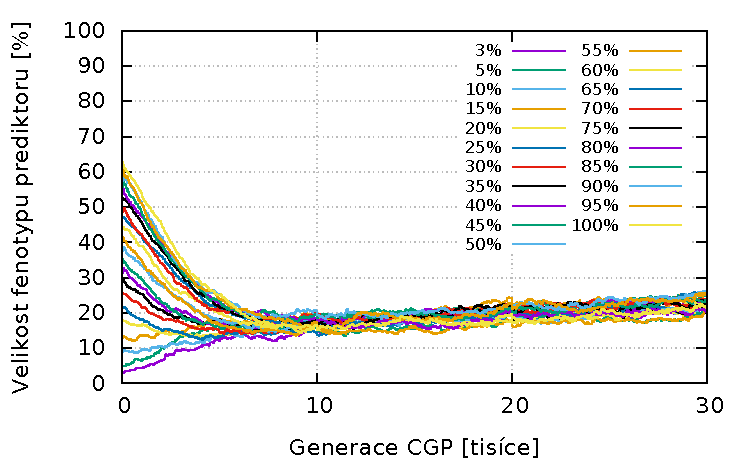
\includegraphics[width=0.9\linewidth]{images/initial-size-5-30kg.pdf}
%     }\\
%     \subfloat[50\% šum sůl a pepř]{
%         \centering
%             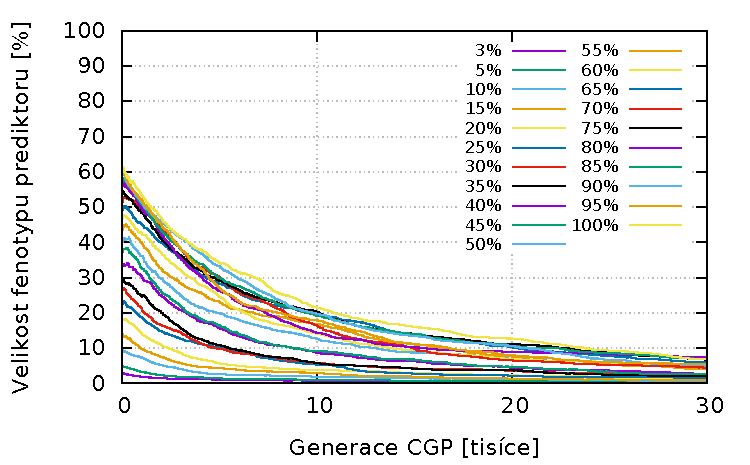
\includegraphics[width=0.9\linewidth]{images/initial-size-50-30kg.pdf}
%     }
%     \caption{Vývoj velikosti prediktorů fitness při různé počáteční velikosti.}
%     \label{fig:InitialSize}
% \end{figure}

\begin{figure}[h]
    \centering
    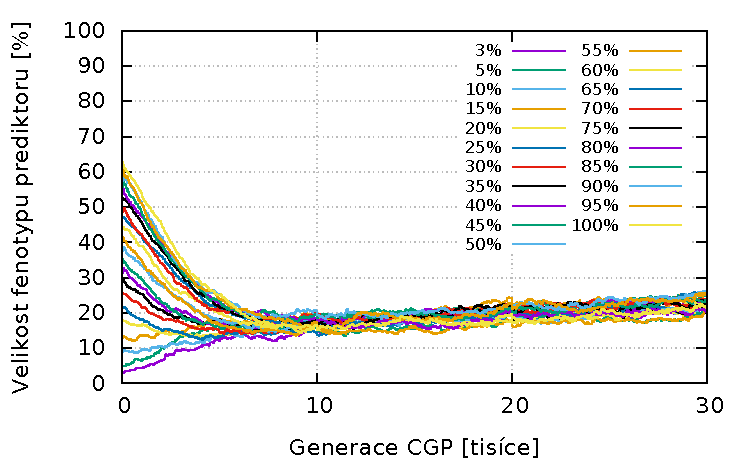
\includegraphics[width=0.95\linewidth]{images/initial-size-5-30kg.pdf}
    \caption{Vývoj velikosti prediktorů fitness při různé počáteční velikosti u 5\% šumu sůl a pepř.}
    \label{fig:InitialSize}
\end{figure}

\subsection{Kvalita filtrů a doba běhu}

Cílem experimentů bylo srovnání koevolučního CGP s adaptivními prediktory fitness ($\mathit{FP_{ADAPT}}$) s koevolučním CGP s prediktory pevné délky ($\mathit{FP_{FIX}}$) a se standardním CGP bez koevoluce ($\mathit{CGP_{STD}}$) s ohledem na kvalitu nalezených obrazových filtrů a na délku běhu programu.

Jak je vidět z výsledků v tabulce \ref{table:quality}, obecně je kvalita filtrů nalezených pomocí $\mathit{FP_{ADAPT}}$ srovnatelná s $\mathit{CGP_{STD}}$ i s nejlepšími výsledky $\mathit{FP_{FIX}}$.

% \begin{figure}[b]
%     \centering
%     \subfloat[Kvalita filtrů]{
%         \centering
%             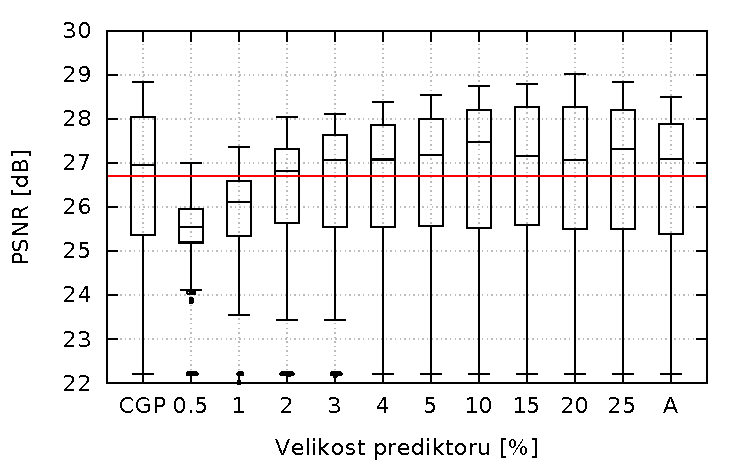
\includegraphics[width=0.85\linewidth]{images/impulse15-30kg-psnr-median.pdf}
%     }\\
%     \subfloat[Čas běhu programu]{
%         \centering
%             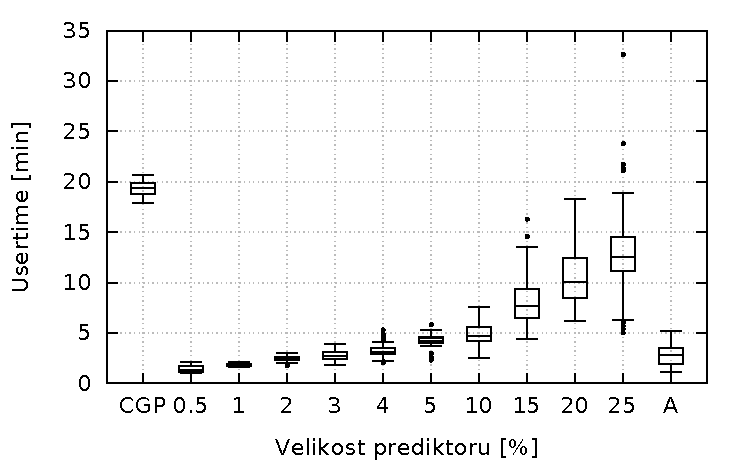
\includegraphics[width=0.85\linewidth]{images/impulse15-30kg-usertime.pdf}
%     }
%     \caption{Srovnání standardního CGP, CGP s koevolucí s prediktory fitness různých délek a koevoluce CGP s prediktory s adaptivní velikostí (A) pro 15\% impulsní šum.}
%     \label{fig:Impulse15}
% \end{figure}


\begin{table*}[t!]
\centering
    \caption{Srovnání kvality nalezených obrazových filtrů pro různé intenzity šumu sůl a pepř pomocí standardního CGP, CGP s koevolucí s prediktory fitness různých délek a s prediktory s adaptivní velikostí (A).}
    \label{table:quality}


    \renewcommand{\arraystretch}{1.1}
    \small
    \color{fixme}
    \begin{tabular}{| c | c | c| c | c | c | c | c | c | c | c | c | c |}
            \hline

                \multirow{3}{1.6cm}{\centering{}Intenzita šumu} & \multirow{3}{*}{} & \multicolumn{11}{c|}{Velikost prediktoru [\% případů fitness]}\\
                \cline{3-13}
                && 0,5 & 1 & 2 & 3 & 4 & 5 & 10 & 15 & 20 & 25 & A \\
                \cline{3-13}
                &&\multicolumn{11}{c|}{PSNR\,[dB]}\\

            \hline\hline



         \multirow{3}{*}{10\,\%}&\textcolor{grayintable}{Min}& \textcolor{grayintable}{15.4} & \textcolor{grayintable}{17.8}  & \textcolor{grayintable}{17.0}
         & \textcolor{grayintable}{15.3} & {\bf \textcolor{grayintable}{20.1}} & \textcolor{grayintable}{15.1}& \textcolor{grayintable}{18.2}\\ %\cline{2-9}

         &Mean& 31.2 & 33.0  & 32.8
         & 32.9 & {\bf 33.2} & 31.0 & 31.7 & 32.9 & {\bf 33.2} & 31.0 & 31.7\\ %\cline{2-9}

         &\textcolor{grayintable}{Max}& \textcolor{grayintable}{36.9} & \textcolor{grayintable}{38.7}  & \textcolor{grayintable}{37.6}
         & \textcolor{grayintable}{38.4} & \textcolor{grayintable}{{\bf 38.9}} & \textcolor{grayintable}{35.6}& \textcolor{grayintable}{37.2}\\ \hline \hline

         \multirow{3}{*}{20\,\%}&\textcolor{grayintable}{Min}& \textcolor{grayintable}{{\bf 18.9}} & \textcolor{grayintable}{15.4}
         & \textcolor{grayintable}{14.5} & \textcolor{grayintable}{14.6} & \textcolor{grayintable}{17.9} & \textcolor{grayintable}{13.9}& \textcolor{grayintable}{17.9} \\ %\cline{2-9}

         &Mean& 25.4 & 26.2  & 25.9
         & 26.1 & {\bf 26.5}& 25.3& 26.2 \\ %\cline{2-9}

         &\textcolor{grayintable}{Max}& \textcolor{grayintable}{30.7} & \textcolor{grayintable}{31.2}  & \textcolor{grayintable}{30.8}
         & \textcolor{grayintable}{31.1} & \textcolor{grayintable}{{\bf 31.5}} & \textcolor{grayintable}{30.6}& \textcolor{grayintable}{30.6} \\ \hline \hline

         \multirow{3}{*}{30\,\%}&\textcolor{grayintable}{Min}& \textcolor{grayintable}{17.7} & \textcolor{grayintable}{13.1}
         & \textcolor{grayintable}{12.6} & \textcolor{grayintable}{13.7} & \textcolor{grayintable}{{\bf 18.8}} & \textcolor{grayintable}{13.0}& \textcolor{grayintable}{18.2} \\ %\cline{2-9}

         &Mean& 22.3 & {\bf 24.9}  & 24.7
         & 24.8 & {\bf 24.9} & 23.7& 24.0 \\ %\cline{2-9}

         &\textcolor{grayintable}{Max}& \textcolor{grayintable}{27.8} & \textcolor{grayintable}{{\bf 28.6}}  & \textcolor{grayintable}{28.5}
         & \textcolor{grayintable}{28.0} & \textcolor{grayintable}{28.0} & \textcolor{grayintable}{28.1}& \textcolor{grayintable}{28.2} \\ \hline \hline

        \multirow{3}{*}{40\,\%} &\textcolor{grayintable}{Min}& \textcolor{grayintable}{16.9} & \textcolor{grayintable}{12.0}  & \textcolor{grayintable}{12.2}
        & \textcolor{grayintable}{11.7} & \textcolor{grayintable}{17.4} & \textcolor{grayintable}{13.3}& \textcolor{grayintable}{{\bf 18.4}} \\ %\cline{2-9}

         &Mean& 20.0 & 20.1  & 20.6
         & 20.8 & {\bf 21.9} & 21.5 & {\bf 21.9} \\ %\cline{2-9}

         &\textcolor{grayintable}{Max}& \textcolor{grayintable}{25.5} & \textcolor{grayintable}{{\bf 27.7}}  & \textcolor{grayintable}{27.2}
         & \textcolor{grayintable}{26.8} & \textcolor{grayintable}{26.9} & \textcolor{grayintable}{26.6}& \textcolor{grayintable}{26.6} \\ \hline\hline

         \multirow{3}{*}{50\,\%} &\textcolor{grayintable}{Min}& \textcolor{grayintable}{16.9} & \textcolor{grayintable}{12.0}  & \textcolor{grayintable}{12.2}
        & \textcolor{grayintable}{11.7} & \textcolor{grayintable}{17.4} & \textcolor{grayintable}{13.3}& \textcolor{grayintable}{{\bf 18.4}} \\ %\cline{2-9}

         &Mean& 20.0 & 20.1  & 20.6
         & 20.8 & {\bf 21.9} & 21.5 & {\bf 21.9} \\ %\cline{2-9}

         &\textcolor{grayintable}{Max}& \textcolor{grayintable}{25.5} & \textcolor{grayintable}{{\bf 27.7}}  & \textcolor{grayintable}{27.2}
         & \textcolor{grayintable}{26.8} & \textcolor{grayintable}{26.9} & \textcolor{grayintable}{26.6}& \textcolor{grayintable}{26.6} \\ \hline\hline

         \multirow{3}{*}{60\,\%} &\textcolor{grayintable}{Min}& \textcolor{grayintable}{16.9} & \textcolor{grayintable}{12.0}  & \textcolor{grayintable}{12.2}
        & \textcolor{grayintable}{11.7} & \textcolor{grayintable}{17.4} & \textcolor{grayintable}{13.3}& \textcolor{grayintable}{{\bf 18.4}} \\ %\cline{2-9}

         &Mean& 20.0 & 20.1  & 20.6
         & 20.8 & {\bf 21.9} & 21.5 & {\bf 21.9} \\ %\cline{2-9}

         &\textcolor{grayintable}{Max}& \textcolor{grayintable}{25.5} & \textcolor{grayintable}{{\bf 27.7}}  & \textcolor{grayintable}{27.2}
         & \textcolor{grayintable}{26.8} & \textcolor{grayintable}{26.9} & \textcolor{grayintable}{26.6}& \textcolor{grayintable}{26.6} \\ \hline\hline

         \multirow{3}{*}{70\,\%} &\textcolor{grayintable}{Min}& \textcolor{grayintable}{16.9} & \textcolor{grayintable}{12.0}  & \textcolor{grayintable}{12.2}
        & \textcolor{grayintable}{11.7} & \textcolor{grayintable}{17.4} & \textcolor{grayintable}{13.3}& \textcolor{grayintable}{{\bf 18.4}} \\ %\cline{2-9}

         &Mean& 20.0 & 20.1  & 20.6
         & 20.8 & {\bf 21.9} & 21.5 & {\bf 21.9} \\ %\cline{2-9}

         &\textcolor{grayintable}{Max}& \textcolor{grayintable}{25.5} & \textcolor{grayintable}{{\bf 27.7}}  & \textcolor{grayintable}{27.2}
         & \textcolor{grayintable}{26.8} & \textcolor{grayintable}{26.9} & \textcolor{grayintable}{26.6}& \textcolor{grayintable}{26.6} \\ \hline\hline

         \multirow{3}{*}{80\,\%} &\textcolor{grayintable}{Min}& \textcolor{grayintable}{16.9} & \textcolor{grayintable}{12.0}  & \textcolor{grayintable}{12.2}
        & \textcolor{grayintable}{11.7} & \textcolor{grayintable}{17.4} & \textcolor{grayintable}{13.3}& \textcolor{grayintable}{{\bf 18.4}} \\ %\cline{2-9}

         &Mean& 20.0 & 20.1  & 20.6
         & 20.8 & {\bf 21.9} & 21.5 & {\bf 21.9} \\ %\cline{2-9}

         &\textcolor{grayintable}{Max}& \textcolor{grayintable}{25.5} & \textcolor{grayintable}{{\bf 27.7}}  & \textcolor{grayintable}{27.2}
         & \textcolor{grayintable}{26.8} & \textcolor{grayintable}{26.9} & \textcolor{grayintable}{26.6}& \textcolor{grayintable}{26.6} \\ \hline

        \end{tabular}
\end{table*}


%--------------------------------------------------------
%--------------------------------------------------------
%--------------------------------------------------------
%--------------------------------------------------------
\section{Závěr}
\label{sec:Conclusions}

\fixme{\blindtext}


%--------------------------------------------------------
%--------------------------------------------------------
%--------------------------------------------------------
%--------------------------------------------------------
\section*{Poděkování}
\label{sec:Acknowledgements}


\fixme{Přátelé, dovolte mi, abych poděkoval všem těm, kteří mně umožnili cenu získat. Byli to v první řadě diváci v první řadě. Ale též diváci v druhé řadě. Diváci ve třetí řadě. Diváci v páté řadě. Přátelé, nemohu zapomenout na diváky ve čtvrté řadě.}


%--------------------------------------------------------
%--------------------------------------------------------
%--------------------------------------------------------
%	REFERENCE LIST
%--------------------------------------------------------
%--------------------------------------------------------
\phantomsection
\bibliographystyle{czechiso}
\inputencoding{latin2}
\bibliography{2015-ExcelFIT-Colearning-bib}

%--------------------------------------------------------
%--------------------------------------------------------
%--------------------------------------------------------
\end{document}
